\documentclass[ngerman,]{article}
\usepackage{lmodern}
\usepackage{amssymb,amsmath}
\usepackage{ifxetex,ifluatex}
\usepackage{fixltx2e} % provides \textsubscript
\ifnum 0\ifxetex 1\fi\ifluatex 1\fi=0 % if pdftex
  \usepackage[T1]{fontenc}
  \usepackage[utf8]{inputenc}
\else % if luatex or xelatex
  \ifxetex
    \usepackage{mathspec}
  \else
    \usepackage{fontspec}
  \fi
  \defaultfontfeatures{Ligatures=TeX,Scale=MatchLowercase}
\fi
% use upquote if available, for straight quotes in verbatim environments
\IfFileExists{upquote.sty}{\usepackage{upquote}}{}
% use microtype if available
\IfFileExists{microtype.sty}{%
\usepackage{microtype}
\UseMicrotypeSet[protrusion]{basicmath} % disable protrusion for tt fonts
}{}
\usepackage[margin=1in]{geometry}
\usepackage{hyperref}
\hypersetup{unicode=true,
            pdfborder={0 0 0},
            breaklinks=true}
\urlstyle{same}  % don't use monospace font for urls
\ifnum 0\ifxetex 1\fi\ifluatex 1\fi=0 % if pdftex
  \usepackage[shorthands=off,main=ngerman]{babel}
\else
  \usepackage{polyglossia}
  \setmainlanguage[]{german}
\fi
\usepackage{longtable,booktabs}
\usepackage{graphicx,grffile}
\makeatletter
\def\maxwidth{\ifdim\Gin@nat@width>\linewidth\linewidth\else\Gin@nat@width\fi}
\def\maxheight{\ifdim\Gin@nat@height>\textheight\textheight\else\Gin@nat@height\fi}
\makeatother
% Scale images if necessary, so that they will not overflow the page
% margins by default, and it is still possible to overwrite the defaults
% using explicit options in \includegraphics[width, height, ...]{}
\setkeys{Gin}{width=\maxwidth,height=\maxheight,keepaspectratio}
\IfFileExists{parskip.sty}{%
\usepackage{parskip}
}{% else
\setlength{\parindent}{0pt}
\setlength{\parskip}{6pt plus 2pt minus 1pt}
}
\setlength{\emergencystretch}{3em}  % prevent overfull lines
\providecommand{\tightlist}{%
  \setlength{\itemsep}{0pt}\setlength{\parskip}{0pt}}
\setcounter{secnumdepth}{0}
% Redefines (sub)paragraphs to behave more like sections
\ifx\paragraph\undefined\else
\let\oldparagraph\paragraph
\renewcommand{\paragraph}[1]{\oldparagraph{#1}\mbox{}}
\fi
\ifx\subparagraph\undefined\else
\let\oldsubparagraph\subparagraph
\renewcommand{\subparagraph}[1]{\oldsubparagraph{#1}\mbox{}}
\fi

%%% Use protect on footnotes to avoid problems with footnotes in titles
\let\rmarkdownfootnote\footnote%
\def\footnote{\protect\rmarkdownfootnote}

%%% Change title format to be more compact
\usepackage{titling}

% Create subtitle command for use in maketitle
\newcommand{\subtitle}[1]{
  \posttitle{
    \begin{center}\large#1\end{center}
    }
}

\setlength{\droptitle}{-2em}

  \title{}
    \pretitle{\vspace{\droptitle}}
  \posttitle{}
    \author{}
    \preauthor{}\postauthor{}
      \predate{\centering\large\emph}
  \postdate{\par}
    \date{08 Februar, 2019}

% Used for placing figures more precisely
\usepackage{float} 
      \let\origfigure\figure 
      \let\endorigfigure\endfigure
      \renewenvironment{figure}[1][2] {
        \expandafter\origfigure\expandafter[H]
      } {\endorigfigure}

\begin{document}

{
\setcounter{tocdepth}{2}
\tableofcontents
}
\newpage

\section{1 Einführung}\label{einfuhrung}

Die Strategie Europa 2020 ist die Agenda der Europäischen Union zur
Förderung von Wachstum und Beschäftigung des gegenwärtigen Jahrzehntes.
Zu der Umsetzung dieses geimsamen europäischen Vorhaben wurden in den
Bereichen Beschäftigung, Forschung, Klimawandel, Armut und soziale
Ausgrenzung nationale Ziele festgelegt, die jährlich im Rahmen von
Fortschrittsberichten beobachtet werden. Insbesondere soll durch eine
Verringerung der Armut, die soziale Eingliederung gefördert werden,
wobei angestrebt wird, mindestens 20 Millionen Menschen vor dem Risiko
der Armut zu bewahren (Statistisches Amt Europäische Kommission 2016).

Im Rahmen dieser Vorhaben setzt die EU ein klares Zeichen zur Bekämpfung
von Armut. Während Armut per se sich nur auf den untersten Teil der
Einkommensverteilung beschränkt, zeigt die Einkommensverteilung das Bild
der gesamten betrachteten Volkswirtschaft. Die OECD weist bereits seit
mehrere Jahren auf die Spreizung der Einkommen hin (OECD 2008; OECD
2015). In dem Report „Growing unequal? Income distribution and poverty
in OECD countries`` befasst sich die Internationale Organisation mit der
Entwicklung der Disparität der Einkommen von 30 Industriestaaten und
zeigt auf, dass mindestens seit der Mitte der 1980er eine geringe,
jedoch kontinuierliche Erhöhung der Ungleichheit stattgefunden hat. Wird
dieser Zeitaum näher betrachtet stellt sich heraus, dass die jeweiligen
Regierungen zwar ihre Ausgaben und Steuern erhöht haben, um dieser
Dynamik entgegenzuwirken, wohingegen der gewünschte Umverteilungseffekt
nur bis Mitte der 1990er Jahre gedämpft werden konnte. In den darauf
folgenden Jahren richtete sich die Umverteilungspolitik weniger gezielt
auf ärmere Haushalte und führte zu einem wesentlich Anstieg der
Ungleichheit. Es wird darauf hingewiesen, dass dies unter anderem
ausschlaggebend für die unteschiedlichen Ausprägungen von Ungleichheit
in den jeweiligen Ländern sei (OECD 2008).

Ersichtlich ist, dass eine effiziente nationale Politik Disparitäten
entgegensteuern kann und Steuern und Transfers wichtige Säule der
Umverteilung sind. Dänemark wird oft als Land dargestellt, dass
Wirtschaftlichkeit und soziale Sicherheit erfolgreich umsetzt. Hier
stellt sich die Frage, ob sich das dänische Model des Wohlfahrtsstaates
auch in der nationalen Einkommensverteilung wiederspiegelt. Um die
Einkommensungleichheit und in diesem Zusammenhang die Entwicklung von
Armut und sozialer Ausgrenzung in Dänemark sichtbar zu machen, wird eine
beurteilende Analyse verschiedener Indikatoren auf Basis von
ausgewählten Daten aus der European Union Statistics on Income and
Living Conditions (EU-SILC) Erhebung im Rahmen dieses Artikels
vorgenommen.

Das nachfolgende Kapitel beschäftigt sich mit den institutionellen und
theoretischen Grundlagen des Landes und ermöglicht es die Auswertung der
Indikatoren in einen Kontext zu betrachten. Behandelt wird in diesem Zug
der dänische Arbeitsmarkt sowie das Steuer und Transfersystem. In
Kapitel 3 liegt der Fokus zum einen auf der Herkunft der verwendeten
Daten und deren Aufbereitung sowie den verschiedenen
Einkommenskonzepten, die zur Analyse herangezogen werden. Außerdem
werden hier die Varianten der Zuteilung von Einkommenskomponenten auf
die Haushaltsmitglieder thematisiert. Die berechneten
Ungleichheitsindikatoren sind in Kapitel 4 visualisiert. Nachdem der
Leser sich nun ein Bild über die Einkommensungleichheit in Dänemark
verschaffen konnte, beschäftigt sich das Kapitel 6 mit der Frage in wie
weit sich Dänemark Richtung dem Ziel der Armutsbekämpfung von der
Strategie Europa 2020 bewegt und ob eine positive Tendenz erkennbar ist.
Zuletzt, werden alle Erkenntnisse und Ergebnisse im Rahmen des
Conclusios reflektiert und zusammengefasst.

\section{2 Institutionelle und theoretische
Grundlagen}\label{institutionelle-und-theoretische-grundlagen}

Im folgenden werden verteilungsrelevante Aspekte des dänischen
Wohlfahrtsstaates erläutert. Diese umfassen das Flexicurity-Prinzip, die
Arbeitslosenunterstützung, aktivierende Maßnahmen, bezahlte Karenz,
Kollektivverträge und Einkommenssteuer.

\subsection{2.1 Das Flexicurity-Prinzip}\label{das-flexicurity-prinzip}

Seit Ausbruch der Ölkrise hatte Dänemark mit anhaltend hohen
Arbeitslosenquoten von rund zehn Prozent zu kämpfen. Um dem
gegenzusteuern und die Arbeitslosigkeit nachhaltig zu senken, wurde das
Flexicurity System schrittweise seit den 1990er Jahren implementiert
(Björklund 2000). Flexicurity ist ein Schachtelwort aus Flexibility und
Security und ist zum einen durch einen lockeren Kündigungsschutz und
andererseits absichernden Maßnahmen für ArbeitnehmerInnen
charakterisiert (OECD 2016a).

\subsection{2.2
Arbeitslosenunterstützung}\label{arbeitslosenunterstutzung}

Vor den Reformen der 1990er Jahre gab es in Dänemark de facto keine
zeitliche Beschränkung der Arbeitslosenunterstützung. Im ersten Schritt
wurde eine maximale Bezugsdauer von sieben Jahren eingeführt. Diese
wurde in weiteren Schritten gesenkt. Seit dem Jahr 2016 beträgt die
maximale Bezugsdauer zwei Jahre und kann im Ausnahmefall auf drei Jahre
verlängert werden. Dies führte dazu, dass heute weniger Personen
Arbeitslosenunterstützung beziehen. Anzumerken ist jedoch, dass
gleichzeitig die Zahl der SozialhilfeempfängerInnen gestiegen ist.
Arbeitslose erhalten in Dänemark einen gewissen Prozentsatz ihres
bisherigen Lohnes, die sogenannte Replacement Rate, von der Versicherung
ausbezahlt. Die Replacement Rate ist nach Einkommen gestaffelt und
beträgt im Durchschnitt rund 60\%. Der Höchstsatz für
NiedrigverdienerInnen kommt auf 90\% in Dänemark. Im OECD-Vergleich sind
beide Prozentsätze Spitzenreiter. Die Ansprüche sind bei einer Höhe, die
in etwa 60\% des Durchschnitsslohns entspricht, gedeckelt und sind somit
für BezieherInnen höherer Einkommen im internationalen Vergleich eher
niedrig (Gaard und Kieler 2005, OECD (2016a)).

\subsection{2.3 Aktivierende Maßnahmen}\label{aktivierende-manahmen}

Ein weiteres Charakteristikum der Flexicurity-Politik stellen sogenannte
aktivierende Maßnahmen dar. Innerhalb von drei Monaten haben Arbeitslose
in Zusammenarbeit mit den Behörden einen Aktionsplan für den beruflichen
Wiedereinstieg zu erstellen. Außerdem können Weiterbildungsprogramme und
die Annahme vermittelter Stellen vorgeschrieben werden. Wird dies
verweigert, so wird die Arbeitslosenunterstützung gekürzt oder
gestrichen. Ziel dieser strikten Maßnahmen ist es die Dauer der
Arbeitslosigkeit zu senken und sicherzustellen, dass die BezieherInnen
bereit sind am Arbeitsmarkt zu partizipieren (Björklund 2000, Gaard und
Kieler (2005)). Insgesamt wendet Dänemark rund 1,8\% des BIPs für aktive
Arbeitsmarktpolitik auf. Auch in diesem Punkt ist Dänemark unter den
OECD Staaten führend (OECD 2016a).

\subsection{2.4 Bezahlte Karenz}\label{bezahlte-karenz}

Zusätzlich zu den bereits genannten Reformen wurden vergleichsweise
großzügige Karenzmodelle ins Leben gerufen. So können ArbeitnehmerInnen
nun bezahlte Bildungs- und Elternkarenz von bis zu einem Jahr in
Anspruch nehmen. Außerdem wurde eine Sabbaticalsystem eingeführt bei dem
ArbeitnehmerInnen 80\% der Arbeitslosenunterstützung erhalten. Die durch
Karenzen freigeworden Stellen werden nach Möglichkeit zwischenzeitlich
mit Arbeitslosen besetzt. Dadurch sollen diese wieder aktiv in den
Arbeitsmarkt integriert werden (Björklund 2000, Gaard und Kieler
(2005)).

\subsection{2.5 Kollektivverträge}\label{kollektivvertrage}

Verhandlungen zwischen den Sozialpartnern haben in Dänemark eine lange
Tradition, jedoch wurde ihre Bedeutung im Rahmen der
Flexicurity-Reformen geschwächt. Während die
Kollektivvertragsverhandlungen früher auf nationaler Ebene durchgeführt
wurden, finden die Verhandlungen seit Beginn der 1980er Jahre auf
Branchenebene statt. In Dänemark wird außerdem zwischen einem Normal-
und einem Mindestlohnsystem unterschieden. Im Normallohnsystem wird der
Vertrag auf Branchenebene verhandelt und kann auf lokaler Ebene nur mehr
geringfügig abgeändert werden, wohingegen das Ergebnis im
Mindestlohnsystem als Untergrenze gilt. Der Anteil der vom
Mindestlohnsystem abgedeckten AbeitnehmerInnen stieg im Zuge der
Reformen um rund 35 Prozentpunkte und lag 1994 bei 85\%. Ein gewisses
Maß an Koordination blieb bei den Verhandlungen dennoch erhalten, da das
verarbeitende Gewerbe üblicherweise mit den Verhandlungen beginnt und
diese als Maßstab für die restlichen Verhandlungen herangezogen werden.
Die Quote der gewerkschaftlich organisierten ArbeiterInnen blieb im Zuge
der Reformen unverändert bei rund 75\% (Björklund 2000).

\subsection{2.6 Einkommenssteuer}\label{einkommenssteuer}

Das dänische Steuersystem unterscheidet grundsätzlich drei
Einkommenskategorien:

\textbf{- Persönliches Einkommen} Löhne und Gehälter, Einkommen aus
selbstständiger Tätigkeit, Pensionen, Arbeitslosenunterstützung

\textbf{- Kapitaleinkommen} Zinserträge und -zahlungen, Dividenden,
imputierte Mieten (Im Falle hoher Zinsaufwendungen kann das
Kapitaleinkommen negativ sein. Imputierte Mieten stellen ein
hypothetisches Einkomman dar. Sie bilden die Ersparnisse ab, die sich
für Personen ergeben, die in ihrem Eigentum wohnen)

\textbf{- Steuerpflichtiges Einkommen} Die Summe von persönlichem und
Kapitaleinkommen abzüglich absetzbarer Ausgaben

Sämtliche ArbeitnehmerInnen in Dänemark zahlen einen Arbeitsmarktbeitrag
von 8\% ihres Bruttoarbeitseinkommens. Dieser wird noch vor der
Berechnung des persönlichen Einkommens abgezogen. Die steuerpflichtigen
Einkommen werden auf nationaler Ebene besteuert. Für Einkommen unter
479.600 Dänischen Kronen (DKK) gilt ein Satz von 10,8\%, für jene
darüber beträgt er 15\%. Gemeinden sind ebenso bemächtigt,
Einkommenssteuer einzuheben. Der Steuersatz der Gemeinden liegt zwischen
22\% und 28\%. Zusätzlich haben ArbeitgeberInnen und ArbeitnehmerInnen
Sozialversicherungsbeiträge zu zahlen (OECD 2018).

Im OECD-Vergleich werden Einkommen relativ stark besteuert (Gaard und
Kieler 2005), was in Kombination mit einer progressiven Steuer eine
starke Umverteilungswirkung der Fiskalpolitik nahelegt. Für
Kapitaleinkommen existieren jedoch zahlreiche Ausnahmen, die diesen
Effekt abschwächen (Ganghof 2007).

\section{3 Methodologie}\label{methodologie}

\subsection{3.1 Daten}\label{daten}

Für eine Analyse der Verteilung der Einkommen aus Erwerbstätigkeit in
Dänemark liefert die Erhebungen „European Union Statistics on Income and
Living Conditions`` (SILC) hinreichend detaillierte Daten.
Ausschließlich für die Inflationsbereinigung werden Daten von EUROSTAT
herangezogen.

Erstmals wurde die EU-SILC Erhebung 2003, basierend auf einer
freiwilligen Vereinbarung zwischen Eurostat und sechs Mitgliedstaaten
(Belgien, Dänemark, Griechenland, Irland, Luxemburg und Österreich)
sowie Norwegen durchgeführt. Inzwischen beteiligen sich neben den
EU-Mitgliedsstaaten auch Norwegen, Island, die Türkei, die Schweiz,
Mazedonien und Serbien an der harmonisierten Stichprobenerhebung von
privaten Haushalten (Eurostat 2019). Mit dem Ziel Armut und sozialer
Ausgrenzung zu beobachten, dient die Erhebung in diesem Zusammenhang zur
Überwachung der Strategie Europa 2020.

Die EU-SILC Erhebung umfasst multidimensionale Mikrodaten zu Einkommen,
Armut, sozialer Ausgrenzung, Wohnraum, Arbeit, Bildung und Gesundheit
und liefert zwei Arten von jährlichen Daten (Eurostat 2013a):

\begin{itemize}
\tightlist
\item
  Querschnittdaten, die einen bestimmten Zeitpunkt beziehungsweise
  Zeitspanne betreffen und
\item
  Längsschnittdaten über Veränderungen im Zeitablauf auf individueller
  Ebene.
\end{itemize}

Anzumerken ist, dass aufgrund der engen Definition von Haushalten,
Personen, die in Anstaltshaushalten oder Gemeinschaftsunterkünften leben
oder ohne festen Wohnsitz sind, nicht in den Daten erfasst werden.

Wie bereits angeführt, nimmt Dänemark seit der Erstherbung teil.
Hervorzuheben ist, dass Dänemark sowie die restlichen nordischen Länder,
Holland und Slowenien zu den einzigen Ländern gehören, in welchen die
Einkommensstatistiken auf vollständigen Registern basieren (Denmark
2019b). Die von Statistics Denmark durchgeführte primärstatistische
Erhebung wird sowohl mit Hilfe von persönlichen (CAPI - Computer
Assisted Personal Interview) und telefonischen (CATI - Computer Assisted
Telephone Interview) Interviews als auch computergestützte (CAWI -
Computer Assisted Web Interviews) Webinterviews realisiert. In 2012
präsentierte Statistics Denmark erstmals seine Erfahrung mit der
Verwendung von CAWI für subjektive Variablen (objektive Informationen
werden aus Registern abgerufen) in EU-SILC (Eurostat 2013b). Vorteilhaft
an diesem Modus der Datenerhebung ist, dass dieser kosteneffizienter
sein kann und die Befragten gemäß ihrer eigenen Geschwindigkeit
antworten können, was wiederum zu höheren Antwortquoten führen kann. Auf
der anderen Seite, kann dieses selbstverwaltende System natürlich zu
missverstandenen Antworten führen, da keine Möglichkeit nach Nachfrage
besteht. Für diese Arbeit sind diese erhobenen Daten jedoch nicht
relevant, da sie in der Pilotphase nur PW010, HS120, HS040 und HS060
betroffen haben (Denmark 2014).

\subsection{3.2 Einkommenskonzepte}\label{einkommenskonzepte}

Im Rahmen der Analyse der Einkommensverteilung in Dänemark werden
folgende drei Einkommenskonzepte verwendet, um etwaige Unterschiede in
der Entwicklung der Indikatoren besser zu verfolgen und Rückschlüsse auf
die Herkunft etwaiger Veränderungen der Lebensbedingungen zu ziehen:

\textbf{1. Faktoreinkommen vor Steuern} Das Faktoreinkommen vor Steuern
setzt sich aus der Summme aus Arbeitseinkommen inklusive Selbstständiger
(PY010G, PY021G, PY050G, HY110G) und Vermögenseinkommen (HY040G, HY090G,
PY080G) zusammen. Dieses Einkommenskonzept erfasst somit nur die
Einkommen aus aktiver Produktion. Unter der Annahme, dass kein
Transfersystem existiert, wird durch dieses Einkommenskonzept eine
direkte Verbindung zu den Arbeitsmärkten geschaffen.

\textbf{2. Nationaleinkommen vor Steuern} Das Nationaleinkommen vor
Steuern inkludiert neben den Komponenten des Faktoreinkommens vor
Steuern noch Pensionen (PY100G) und Arbeitslosengeld (PY090G). In diesem
Einkommenskonzept werden nur arbeitsrelevante Transferzahlungen
hinzugezogen, um eine etwaige Verzerung aufgrund von Veränderungen in
der Altersstrukturen (Personen in Pension mit keinem beziehungsweise
geringem Faktoreinkommen) zu berücksichtigen. Unterschiede in der
Entwicklung von Faktoreinkommen vor Steuern und Nationaleinkommen vor
Steuern legen Reformen im Bereich der Arbeitslosen- beziehungsweise
öffentlichen Pensionsversicherung nahe.

\textbf{3. Verfügbares Einkommen nach Steuern} Das verfügbare Einkommen
nach Steuern inkludiert neben den Komponenten des Nationaleinkommens vor
Steuern alle anderen erhaltenen Transferzahlungen (PY110G, PY120G,
PY130G, PY140G, HY050G, HY060G, HY070G, HY080G) abzüglich aller direkten
Steuern und Sozialversicherungsabgaben (HY120G, HY130G, HY140G).
Schließlich zeigt das verfügbare Einkommen nach Steuern wie der Staat
die Höhe und Verteilung der verfügbaren Einkommen durch (weitere)
monetäre Transfers beeinflussen kann.

\subsection{3.3 Allokation der
Haushaltskomponenten}\label{allokation-der-haushaltskomponenten}

Wie aus den oberen Konzepten erkenntlich ist, gibt es sowohl Variablen
auf Personen- (PY010G) als auch Haushaltsebene (HY110G). Die
Einkommenskomponenten beziehungsweise Steuern, die nur auf
Haushaltsebene verfügbar sind, werden auf die einzelnen
Haushaltsmitgleider aufgeteilt. Die Allokation erfolgt nach folgenden
zwei Aufschlüsselungsmethoden:

\textbf{1. P1 Eurostat } Hierbei werden alle Einkommen eines Haushaltes
in einem gleichem Maß auf die äquivalten Haushaltsmitglieder aufgeteilt.

\textbf{2. P2 wid.world } Im Gegensatz zu der vorhergehenden Variante,
werden hier nicht mehr alle in einem Haushalt lebenden Personen in das
Sample genommen. Hier erfolgt eine Ausschließung von Personen unter 20
Jahren. Außerdem wird lediglich die Einkommensvariable, die nur auf
Haushaltsebene verfügbar ist durch die Anzahl der Haushaltsmitglieder
(\textgreater{}20) gleichmäßig auf alle Haushaltsmitgleider aufgeteilt;
die persönlichen Einkommen bleiben den jeweiligen Personen vorbehalten.

\section{4 Ungleichheitsindikatoren}\label{ungleichheitsindikatoren}

Im Folgenden wird die Einkommensverteilung in Dänemark anhand von
mehreren standardisierten Indikatoren für den Zeitraum 2004-2017
analysiert, um Rückschlüsse über die Ungleichheit des Landes zu geben.

In diesem Abschnitt liegt der Fokus der Auswertung auf P1. Begründet
wird dies dadurch, dass die Daten über Steuern nur auf Haushaltsebene
verfügbar sind. Würden wir beispielsweise die Variante P2 heranziehen,
wenn wir eine geringverdienende Frau mit sehr gut verdienenden Mann
betrachten, stellt sich heraus, dass sie neben ihrem geringen Einkommen
die Steuerlast ihres Mannes in der Einkommensverteilung mitträgt.
Sämtliche Gesamtübersichten der berechneten Indikatoren befinden sich
für beide Allokationsvarianten, sprich P1 und P2, im Appendix.

\subsection{4.1 Mittelwert und Median}\label{mittelwert-und-median}

Für einen ersten Eindruck, werden Mittelwert und Median Einkommen näher
betrachtet, da diese Aufschluss über die Schiefe der Verteilungsfunktion
geben. Die Abbildung 1 zeigt die Entwicklung des Median- und
Durchschnittseinkommens nach Steuern (Einkommenskonzept 3) seit 2004.

\begin{figure}
\centering
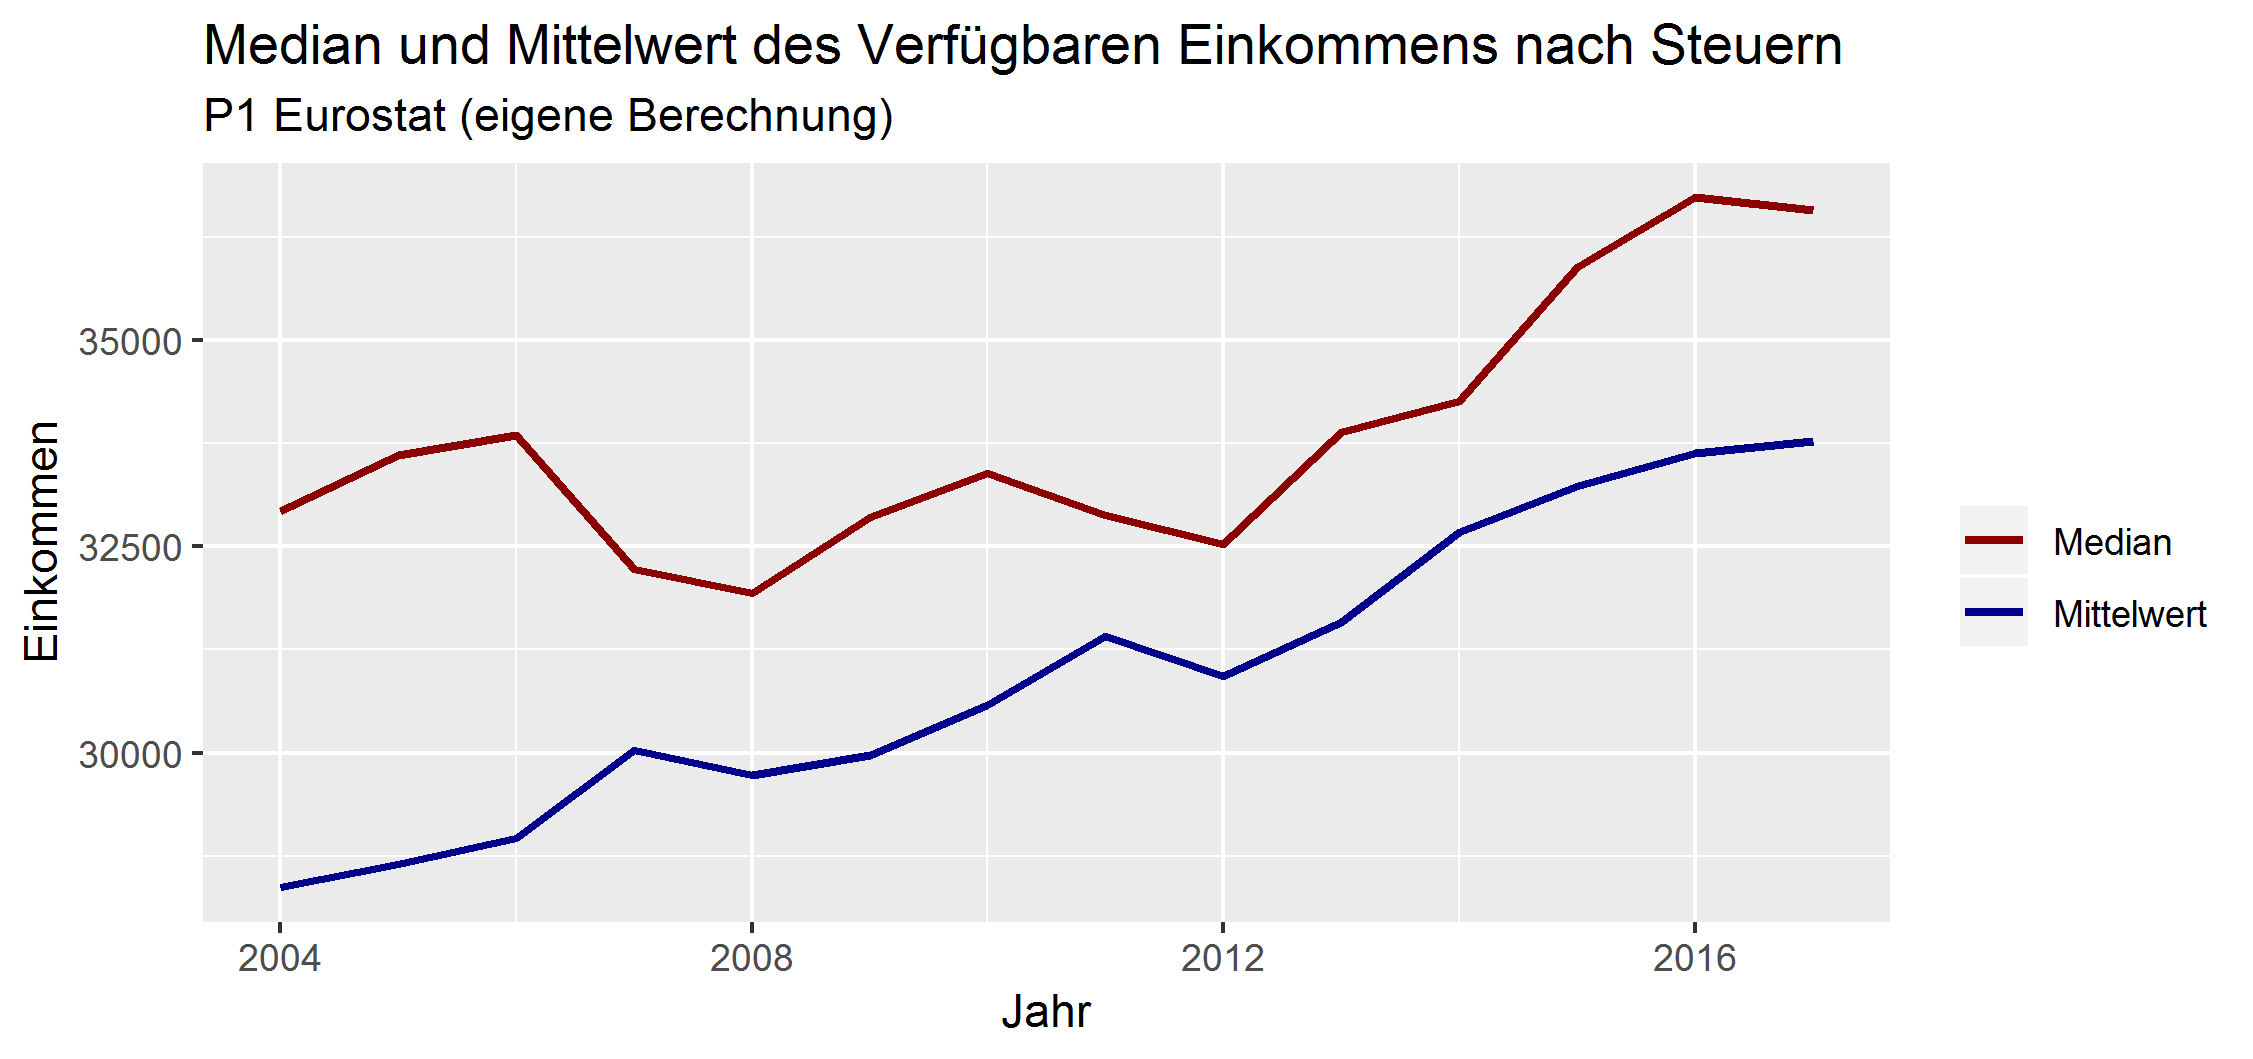
\includegraphics[width=0.65000\textwidth]{img/medmit.png}
\caption{Median und Mittelwert, 2004-2017}
\end{figure}

Es fällt sofort ins Auge, dass beide Werte über den Zeitverlauf stark
gestiegen sind. Die Betrachtung des durchschnittlichen Jahreseinkommen
zeigt von 2004 bis 2017 eine Erhöhung von rund 28.371 DKK auf 33.776
DKK, was knapp 20\% entspricht. Für das Medianeinkommen beträgt die
Erhöhung in diesem Fall lediglich rund 15\%.

Da das Durchschnittseinkommen deutlich unter dem Medianeinkommen liegt,
kann man daraus schließen, dass die Einkommensverteilung eine
rechtsschiefe Dichtefunktion ausweist. Dies ist charakteristisch für
eine Einkommensverteilung. Aus der Grafik ist gut ersichtlich, dass
Dänemark nicht unverschohnt von der Wirtschafts- und Finanzkrise 2008
geblieben ist und sich diese auf die Einkommen privater Haushalte
negativ ausgewirkt hat. Diese Annahme wird durch Denmark (2019a)
bestätigt, die auch zeigen, dass Dänemark die Folgen der Krise langsamer
kompensiert hat als dessen Nachbarländer.

\subsection{4.2 Gini Koeffizient}\label{gini-koeffizient}

Durch den Vergleich von Median und Mittelwert lassen sich nur beschränkt
Schlüsse auf die Einkommensverteilung ziehen. Ein detaillierteres Bild
liefert der Gini Koeffizient. Entspricht der Gini einem Wert von Null,
liegt vollständige Gleichverteilung vor, nimmt er 1 an, so gehört einer
Person das ganze Vermögen in der Gesellschaft.

\begin{figure}
\centering
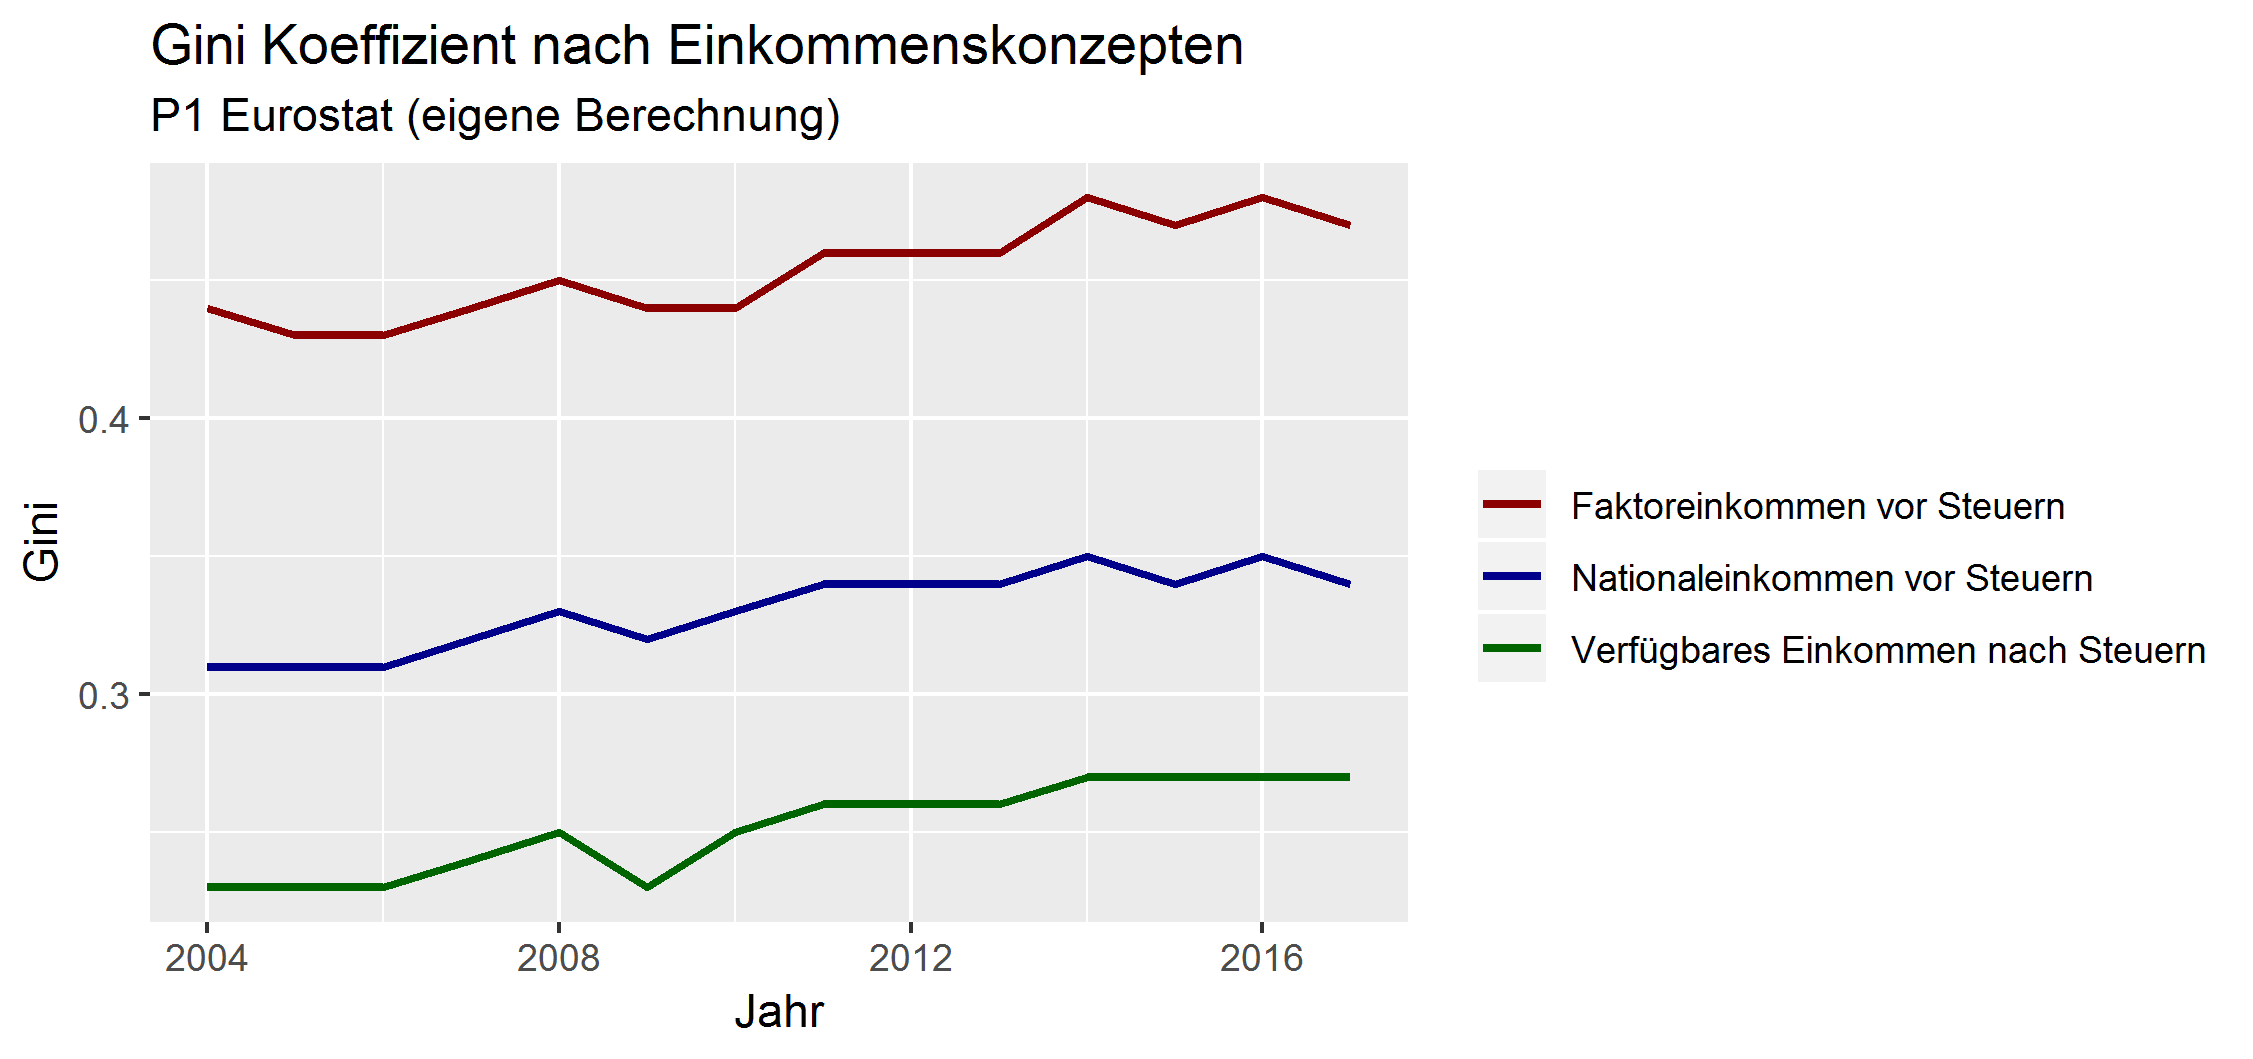
\includegraphics[width=0.65000\textwidth]{img/gini.png}
\caption{Gini-Index, 2004-2017}
\end{figure}

Abbildung 2 zeigt die Entwicklung des Gini Koeffizienten nach den drei
Einkommenskonzepten seit 2004. Klar ersichtlich ist, dass die
staatlichen Umverteilungssysteme die\\
Einkommensungleichheit stark sinken lassen. Dies sieht man beim
Vergleich des Ginis für das verfügbare Einkommen nach Steuern mit den
beiden anderen Einkommenskonzepten. Sowohl Arbeitslosenunterstützung und
Pensionen als auch Steuer- und Transfersysteme lassen die Ungleichheit
in einem größeren Ausmaß sinken. Für das Jahr 2017 bedeutet dies eine
Senkung von insgesamt 20\%. Insgesamt ist im Zeitverlauf die
Ungleichheit in Dänemark gestiegen. Außerdem zeigt Tabelle 5 aus dem
Appendix, dass der Gini-Koeffizient nach der Berechnung P2 für alle
Zeitpunkte deutlich höher ist. Dies erfolgt aus der Konstruktion der
Allokationsvariante.

\subsection{4.3 P80/P20 Verhältnis}\label{p80p20-verhaltnis}

Das P80/P20 Verhältnis stellt den Mittelwert der oberen 20\% relativ zu
den unteren 20\% der EinkommensbezieherInnen gegenüber.

\begin{figure}
\centering
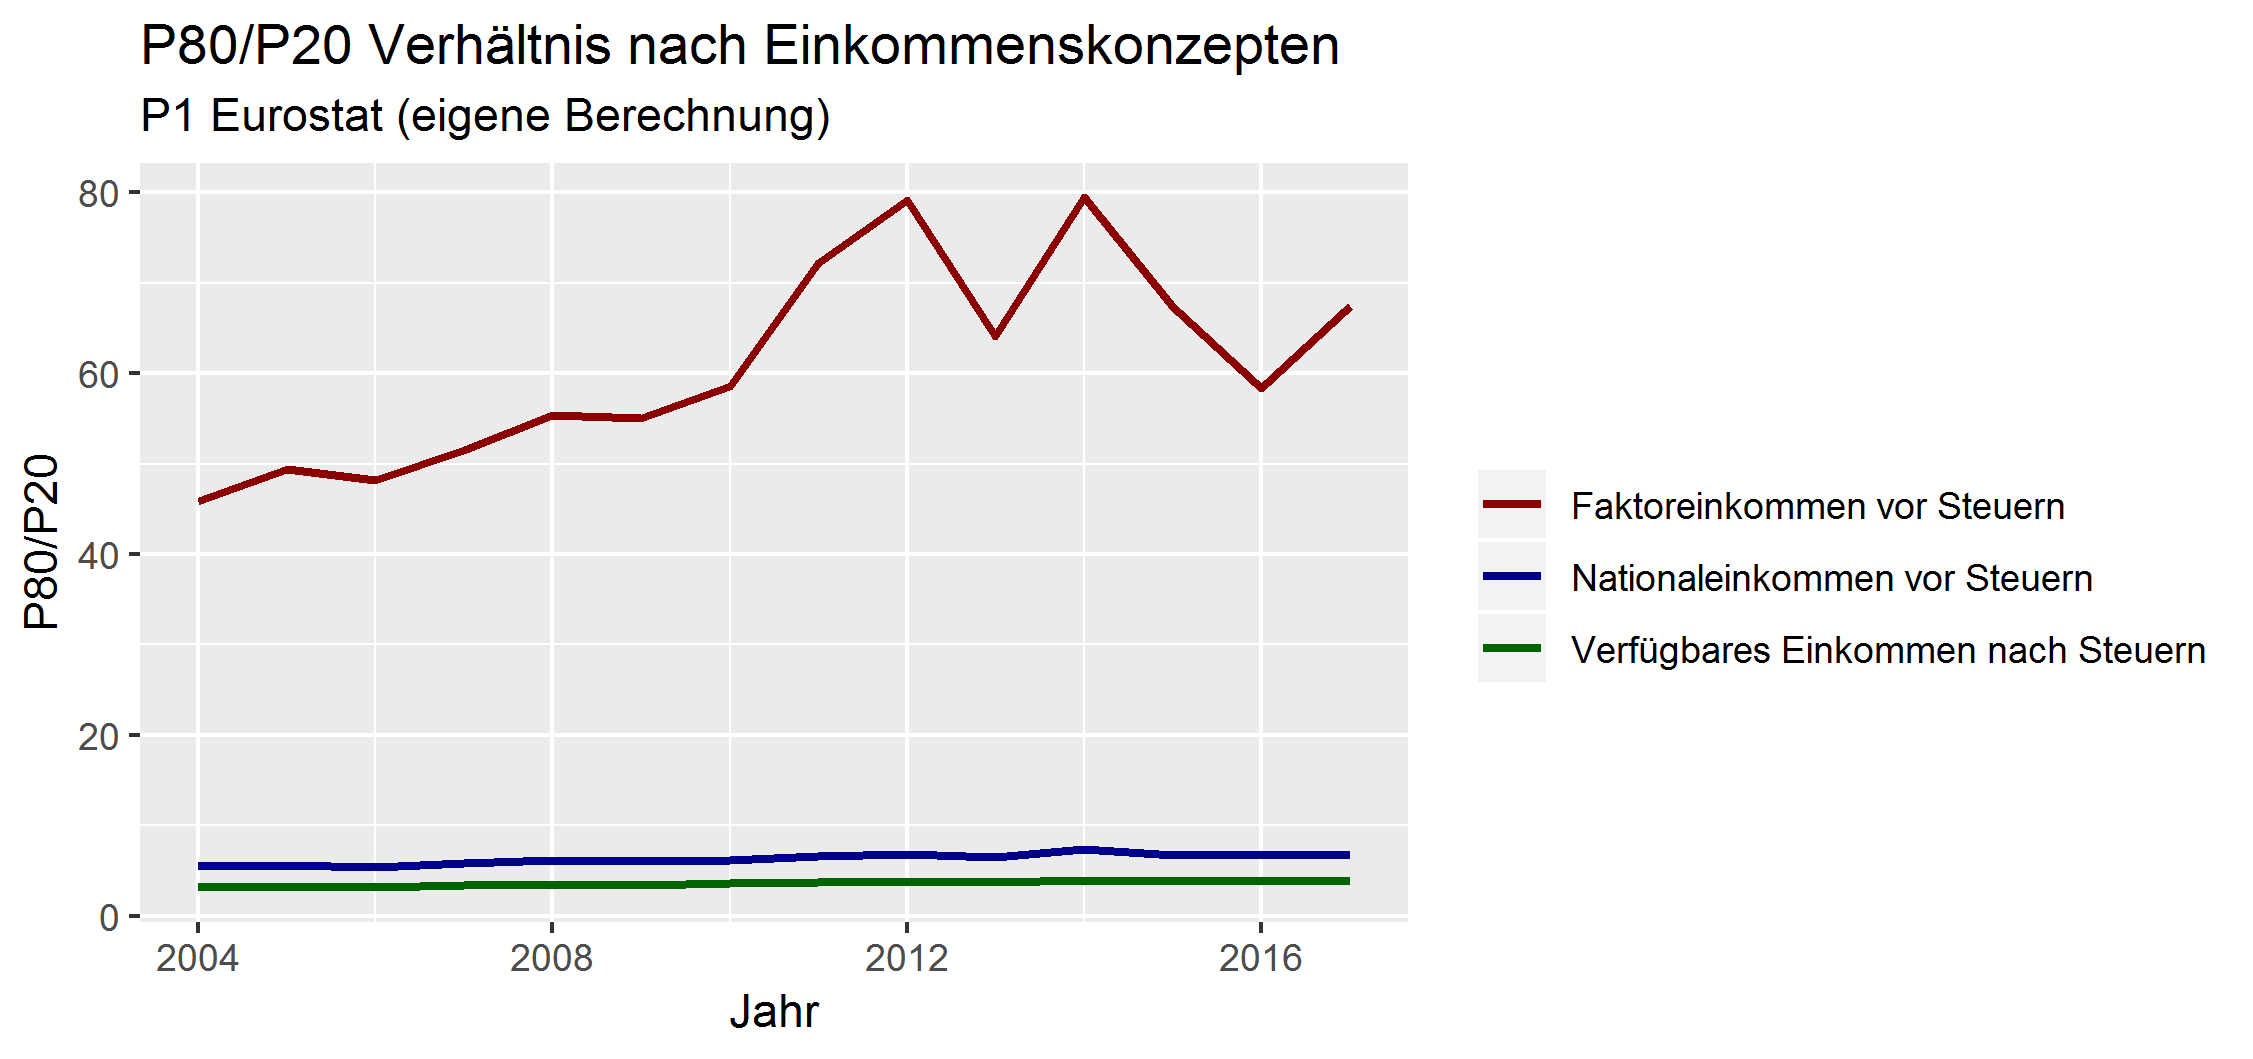
\includegraphics[width=0.65000\textwidth]{img/8020.png}
\caption{P80/P20 Verhältnis, 2004-2017}
\end{figure}

Um das P80/P20 Verhältnis für Dänemark zu illustrieren, werden die drei
verschiedenen Einkommenskonzepte über den Zeitrahmen 2004-2017 in
Abildung 3 betrachtet. Unter der Annahme, dass der mittlere
Einkommensteil in diesem Verhältnis ausgeblendet wird, ist dieses Maß
wesentlich sensitives bei Veränderungen an den Rändern der Verteilung.
Für die Auswertung von Dänemark sieht man, dass der Unterschied zwischen
Faktoreinkommen vor Steuern und dem verfügbaren Einkommen nach Steuern
zu einem größeren Teil durch das progressive Steuersystem erklärbar ist.
Dieses Verteilungsmaß zeigt einen leicht steigenden Trend zu mehr
Ungleichheit. Für die verfügbaren Einkommen beträgt das P80/P20
Verhältnis rund 4\%. Dies bedeutet, dass eine Person aus den top 20\% im
Durchschnitt das vier-fache des Einkommens einer Person der unteren 20\%
verdient.

\subsection{4.4 Top 10\% Anteil}\label{top-10-anteil}

Der Top 10\% Anteil gibt Auskunft ob die Einkommen an der Spitze davon
laufen.

\begin{figure}
\centering
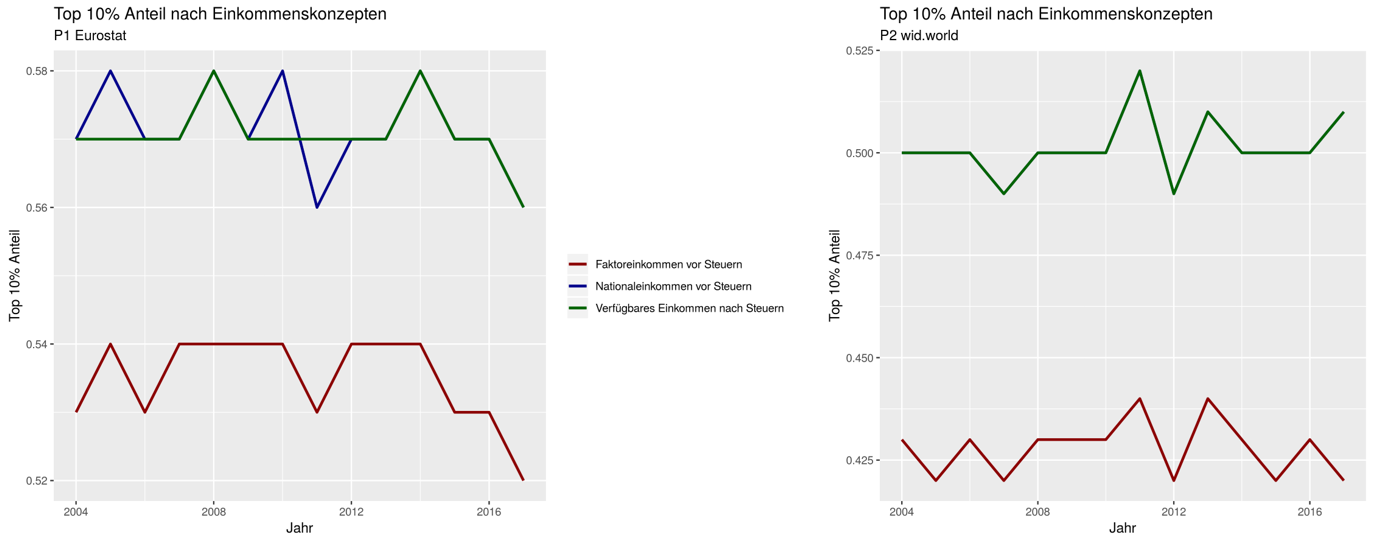
\includegraphics[width=1.00000\textwidth]{img/toptenfull.png}
\caption{Top 10\% Anteil nach P1 und P2, 2004-2017}
\end{figure}

Abbildung 4 zeigt die Entwicklung des Top 10\% Anteils nach den drei
Einkommenskonzepten für beide Allokationsvarianten. Der Anteil der Top
10\% ist für die jeweiligen Einkommenskonzepte im Zeitverlauf konstant.
Für die verfügbaren Einkommen liegt dieser Wert für P1 im Durchschnitt
bei 0,57 und bei P2 0,50. Dies bedeutet, dass die Top-Verdiener die
Hälfte des Gesamteinkommens beziehen. Die Einkommenskonzepte
Nationaleinkommen vor Steuern und das verfügbare Einkommen nach sind in
beiden Varianten P1 und P2, wie zu erwarten, nahezu ident. Da die Werte
der Top-10\% über den Zeitverlauf konstant erscheinen, lässt ich daraus
schließen, dass die Umverteilungslast von anderen Einkommensschichten
getragen wird.

\section{5 Armut in Dänemark}\label{armut-in-danemark}

Die Strategie Europa 2020 hat es sich zum Ziel gesetzt, mindestens 20
Millionen Menschen vor dem Risiko der Armut zu bewahren. Dementsprechend
stehen die jeweiligen Staaten mit ihren abgestimmten nationalen
Benchmarks vor einer großen gemeinschaftlichen Herausforderung . Im
folgenden wird analysiert, in wie weit sich Dänemark Richtung dem Ziel
der Armutsbekämpfung von der Strategie Europa 2020 bewegt und ob eine
positive Tendenz erkennbar ist.

\subsection{5.1 Armutsgefährdungsquote}\label{armutsgefahrdungsquote}

Ein wertvoller Indikator hierbei ist die Armutsgefährdungsquote. Diese
zeigt den Anteil jener, die aufgrund ihres relativ geringen Einkommens
von Armut und sozialer Ausgrenzung bedroht sind. Nach dem EU-Standard
entspricht diese Quote dem Anteil der Personen, deren
Äquivalenzeinkommen weniger als 60\% des Medians der Äquivalenzeinkommen
der Bevölkerung beträgt. Daraus ist ersichtlich, dass die
Armutsgefährdungsquote nur relativ betrachtet werden kann und häufig
(nicht zwanghaft) auf einen niedrigen Lebensstandard der Betroffenen
hindeutet.

\begin{figure}
\centering
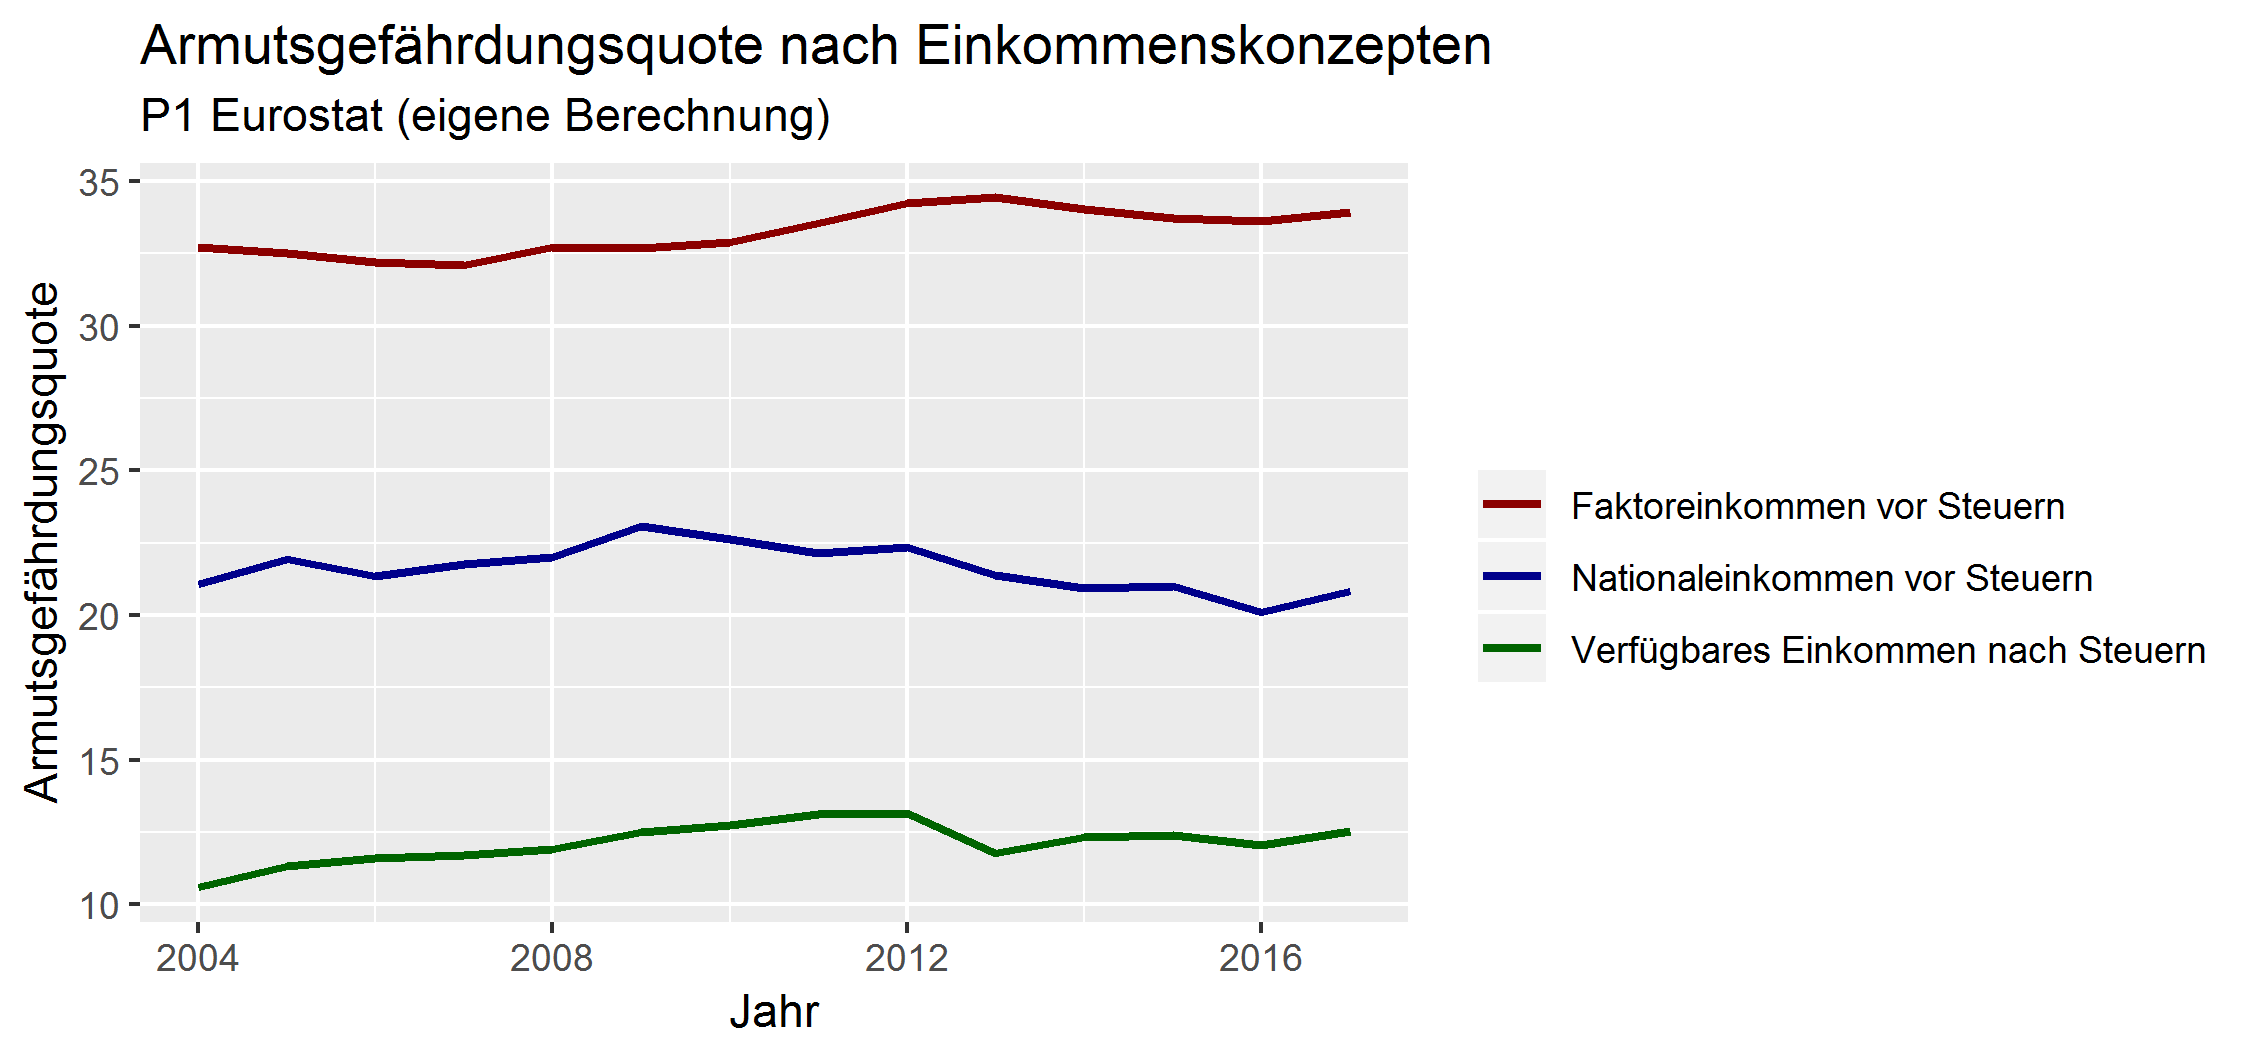
\includegraphics[width=0.90000\textwidth]{img/arpr.png}
\caption{Armutsgefährdungsquote, 2004-2017}
\end{figure}

Abbildung 4 zeigt die Entwicklung der Armutsgefährdungsquote nach den
drei Einkommenskonzepten für P1. Insgesamt ist die
Armutsgefährdungsquote über den Zeitverlauf gestiegen. Unter alleiniger
Betrachtung des verfügbaren Einkommens nach Steuern ist hier ein Anstieg
von 1,95\% in dem Zeitraum 2004-2017 beobachtbar. Zwar kann Dänemark im
EU-Vergleich eine gerine Armutsgefährdungsquote per se aufweisen,
dennoch bewegt sich das Land noch nicht in die richtige Richtung für die
Strategie Europa2020. Dies bedeutet, dass die 2010 von Europäischen Rat
verabschiedeten Zielvorgaben die bis 2020 erfüllt werden sollten, in
weitere Ferne rücken. Vergleichen wir 2010 mit den neuesten Werten von
2017 (im Detail siehe Appendix) ist kaum eine Veränderung der Rate
beobachtbar.

\subsection{5.2 Zerlegung der
Armutsgefährdungsquote}\label{zerlegung-der-armutsgefahrdungsquote}

Die Zerlegung der Armutsgefährdungsquote nach Geschlecht zeigt folgendes
Bild:

\begin{longtable}[]{@{}lrr@{}}
\caption{Zerlegung Armutsgefährdungsquote nach Geschlecht
(2015)}\tabularnewline
\toprule
Einkommenskonzept & Weiblich & Männlich\tabularnewline
\midrule
\endfirsthead
\toprule
Einkommenskonzept & Weiblich & Männlich\tabularnewline
\midrule
\endhead
i13 & 0.5000402 & 0.4999598\tabularnewline
i23 & 0.5575462 & 0.4424538\tabularnewline
\bottomrule
\end{longtable}

Die Tabelle zeigt welcher Prozentsatz an Armutsgefährdeten nach den
beide Berechnungsmethoden weiblich, bzw. männlich ist. Auch hier ist ein
klarer Unterschied zwischen P1 und P2 erkennbar. Nach P2 ist die
Mehrheit der Armutsgefährdeten weiblich, während das Ergbnis von P2
diesen Schluss nicht zulässt.

Die Zerlegung der Armutsgefährdungsquote nach Alter zeigt folgendes
Bild:

\begin{longtable}[]{@{}lrr@{}}
\caption{Zerlegung Armutsgefährdungsquote nach Alter
(2015)}\tabularnewline
\toprule
Einkommenskonzept & Unter 30 & Älter\tabularnewline
\midrule
\endfirsthead
\toprule
Einkommenskonzept & Unter 30 & Älter\tabularnewline
\midrule
\endhead
i13 & 0.5347716 & 0.4652284\tabularnewline
i23 & 0.4325957 & 0.5674043\tabularnewline
\bottomrule
\end{longtable}

Diese Tabelle zeigt nur auf den ersten Blick ein uneindeutiges Bild.
Zwar ist je nach Berechnungsmethode eine Gruppe innerhalb der
Armutsgefährdeten in der Mehrheit, jedoch sind die
Unter-Dreißig-Jährigen in der Grundgesamtheit stark unterrepräsentiert.
Daraus können wir schließen, dass Unter-Dreißig-Jährige in Dänemark
besonders von Armut gefährdet sind.

\section{6 Conclusio}\label{conclusio}

Insgesamt zeigen sämtliche Ergebnisse die starke umverteilende Wirkung
des dänischen Transfer- und Steuersystems. Ohne diesen Mechanismus wären
die Einkommen in Dänemark deutlich ungleicher verteilt. Zusammenfassend
lässt sich sagen, dass die Ungleichheit in Dänemark grundsätzlich
niedrig, im speziellen Beobachtungszeitraum, 2004-2017, jedoch leicht
gestiegen ist. Dieses Ergebnis ist im Einklang mit dem aktuellen Stand
der Forschung und dem internationalen Trend (OECD 2016a, Causa u.~a.
(2016)). Die genauen Ursachen für diese Entwicklung lassen sich mit den
vorliegenden Daten vermutlich nicht identifizieren. Fest steht jedoch,
dass die schrittweise Verschärfung der Bestimmungen zur
Arbeitslosenunterstützung und damit der Rückgang der BezieherInnen von
Arbeitslosenunterstützung mit einem Anstieg an SozialhilfeempfängerInnen
und FrühpensionistInnen einherging (Gaard und Kieler 2005, OECD
(2016a)). Für uns lässt sich daraus schließen, dass das
Flexicurity-System Dänemarks, das Problem der Arbeitslosigkeit nur
oberflächlich zu lösen scheint.

Des weiteren konnten wir einen Anstieg der Armutsgefährungsquote in
Dänemark über den Beobachtungszeitraum feststellen, wobei Frauen und
Unter-Dreißig-Jährige in dieser Gruppe überrepräsentiert sind.
Anzumerken ist, dass dieser Effekt für Frauen nicht eindeutig ist. Auch
dieses Ergebnis deckt sich mit der bestehenden Literatur (OECD (2016b)).
Für die Agenda der EU, Europa2020, ist dies kein Fortschritt von
Dänemark im Bereich Armutsbekämpfung.

Anzumerken ist, dass die Ergebnisse dieser Arbeit nur einen kleinen Teil
der Einkommensungleichheit und Armut in Dänemark repräsentieren. Für
eine tiefergehende Analyse bedarf es noch mehr Forschung und zusätzliche
Daten. Besonders interessant wäre in diesem Sinne eine genauere
Betrachtung der Haushaltsstruktur.

\newpage

\section{Appendix}\label{appendix}

\textbf{Legende}

\begin{itemize}
\tightlist
\item
  i11: Faktoreinkommen vor Steuern nach P1 Eurostat
\item
  i12: Nationaleinkommen vor Steuern nach P1 Eurostat
\item
  i13: Verfügbares Einkommen nach Steuern nach P1 Eurostat
\item
  i21: Faktoreinkommen vor Steuern nach P2 wid.world
\item
  i22: Nationaleinkommen vor Steuern nach P2 wid.world
\item
  i23: Verfügbares Einkommen nach Steuern nach P2 wid.world
\item
  DS: Denmark Statistics
\end{itemize}

~

\textbf{Gesamtübersichten der Indikatoren}

\begin{longtable}[]{@{}rrrrrrr@{}}
\caption{Gesamtübersicht Mittelwert}\tabularnewline
\toprule
Jahr & i11 & i12 & i13 & i21 & i22 & i23\tabularnewline
\midrule
\endfirsthead
\toprule
Jahr & i11 & i12 & i13 & i21 & i22 & i23\tabularnewline
\midrule
\endhead
2004 & 34430.34 & 40891.98 & 28370.61 & 32915.76 & 38678.16 &
27293.91\tabularnewline
2005 & 34474.53 & 40681.39 & 28651.63 & 33033.01 & 38532.54 &
27482.93\tabularnewline
2006 & 34915.35 & 41210.60 & 28964.12 & 33469.94 & 39112.04 &
27832.18\tabularnewline
2007 & 36614.52 & 42788.87 & 30037.79 & 32767.63 & 37975.43 &
33077.26\tabularnewline
2008 & 36455.49 & 42404.63 & 29727.99 & 32664.52 & 37697.24 &
32687.69\tabularnewline
2009 & 36382.80 & 42570.60 & 29976.66 & 32939.52 & 38202.15 &
33342.34\tabularnewline
2010 & 36123.19 & 42613.77 & 30575.51 & 32705.73 & 38206.55 &
33734.08\tabularnewline
2011 & 36733.95 & 43568.14 & 31416.40 & 33424.57 & 39197.48 &
34724.54\tabularnewline
2012 & 35532.70 & 42582.28 & 30931.32 & 33039.80 & 39163.04 &
34834.15\tabularnewline
2013 & 36410.88 & 43735.41 & 31577.54 & 34227.54 & 40682.65 &
36100.98\tabularnewline
2014 & 37655.67 & 45537.10 & 32676.44 & 36375.47 & 43379.57 &
31693.98\tabularnewline
2015 & 38132.84 & 46178.73 & 33226.56 & 36793.45 & 43959.14 &
32104.97\tabularnewline
2016 & 39909.14 & 47567.60 & 33624.55 & 38451.81 & 45292.76 &
32772.00\tabularnewline
2017 & 39785.66 & 47722.42 & 33775.70 & 38356.84 & 45432.31 &
32784.68\tabularnewline
\bottomrule
\end{longtable}

\begin{longtable}[]{@{}rrrrrrrr@{}}
\caption{Gesamtübersicht Median}\tabularnewline
\toprule
Jahr & i11 & i12 & i13 & i21 & i22 & i23 & DS\tabularnewline
\midrule
\endfirsthead
\toprule
Jahr & i11 & i12 & i13 & i21 & i22 & i23 & DS\tabularnewline
\midrule
\endhead
2004 & 33157.57 & 37304.94 & 26361.07 & 32930.26 & 35231.47 & 24137.49 &
171632\tabularnewline
2005 & 33386.58 & 37659.82 & 27127.42 & 33598.70 & 35976.64 & 24701.63 &
176769\tabularnewline
2006 & 33750.79 & 38127.54 & 27321.69 & 33842.41 & 36321.14 & 24928.25 &
182207\tabularnewline
2007 & 34847.34 & 38895.62 & 27803.14 & 32228.55 & 35254.31 & 30140.08 &
186859\tabularnewline
2008 & 34428.25 & 37702.56 & 27280.28 & 31938.67 & 34690.18 & 29517.02 &
191690\tabularnewline
2009 & 35616.96 & 39030.71 & 28248.49 & 32858.34 & 35807.18 & 30724.11 &
196670\tabularnewline
2010 & 34407.02 & 38749.23 & 28508.38 & 33387.50 & 36204.45 & 31416.38 &
209596\tabularnewline
2011 & 34849.23 & 39571.97 & 28865.47 & 32876.25 & 36828.55 & 31857.22 &
213213\tabularnewline
2012 & 33096.32 & 38489.05 & 28229.03 & 32527.04 & 36583.24 & 31593.33 &
217063\tabularnewline
2013 & 33581.99 & 39159.14 & 28470.82 & 33880.42 & 37709.14 & 32559.22 &
221207\tabularnewline
2014 & 33791.30 & 39838.12 & 29256.93 & 34255.25 & 38823.39 & 27380.34 &
226698\tabularnewline
2015 & 35097.38 & 40867.56 & 29862.23 & 35880.45 & 39682.86 & 27911.45 &
230127\tabularnewline
2016 & 35063.49 & 41051.65 & 30068.52 & 36722.67 & 40376.15 & 28315.64 &
234523\tabularnewline
2017 & 35571.66 & 42095.37 & 30307.75 & 36574.66 & 40879.46 & 28565.74 &
240315\tabularnewline
\bottomrule
\end{longtable}

\begin{longtable}[]{@{}rrrrrrrr@{}}
\caption{Gesamtübersicht Gini-Koeffizienten}\tabularnewline
\toprule
Jahr & i11 & i12 & i13 & i21 & i22 & i23 & DS\tabularnewline
\midrule
\endfirsthead
\toprule
Jahr & i11 & i12 & i13 & i21 & i22 & i23 & DS\tabularnewline
\midrule
\endhead
2004 & 0.44 & 0.31 & 0.23 & 0.47 & 0.34 & 0.32 & 0.25\tabularnewline
2005 & 0.43 & 0.31 & 0.23 & 0.47 & 0.34 & 0.31 & 0.26\tabularnewline
2006 & 0.43 & 0.31 & 0.23 & 0.46 & 0.34 & 0.31 & 0.26\tabularnewline
2007 & 0.44 & 0.32 & 0.24 & 0.49 & 0.38 & 0.34 & 0.27\tabularnewline
2008 & 0.45 & 0.33 & 0.25 & 0.50 & 0.39 & 0.35 & 0.28\tabularnewline
2009 & 0.44 & 0.32 & 0.23 & 0.49 & 0.38 & 0.34 & 0.27\tabularnewline
2010 & 0.44 & 0.33 & 0.25 & 0.49 & 0.37 & 0.34 & 0.27\tabularnewline
2011 & 0.46 & 0.34 & 0.26 & 0.51 & 0.39 & 0.35 & 0.28\tabularnewline
2012 & 0.46 & 0.34 & 0.26 & 0.50 & 0.38 & 0.34 & 0.27\tabularnewline
2013 & 0.46 & 0.34 & 0.26 & 0.51 & 0.38 & 0.34 & 0.28\tabularnewline
2014 & 0.48 & 0.35 & 0.27 & 0.51 & 0.39 & 0.35 & 0.28\tabularnewline
2015 & 0.47 & 0.34 & 0.27 & 0.50 & 0.37 & 0.35 & 0.29\tabularnewline
2016 & 0.48 & 0.35 & 0.27 & 0.51 & 0.38 & 0.36 & 0.29\tabularnewline
2017 & 0.47 & 0.34 & 0.27 & 0.51 & 0.38 & 0.35 & 0.29\tabularnewline
\bottomrule
\end{longtable}

\begin{longtable}[]{@{}rrrrrrrr@{}}
\caption{Gesamtübersicht P80/P20 Verhältnis}\tabularnewline
\toprule
Jahr & i11 & i12 & i13 & i21 & i22 & i23 & DS\tabularnewline
\midrule
\endfirsthead
\toprule
Jahr & i11 & i12 & i13 & i21 & i22 & i23 & DS\tabularnewline
\midrule
\endhead
2004 & 45.85 & 5.54 & 3.19 & 86.91 & 7.14 & 5.39 & 3.54\tabularnewline
2005 & 49.39 & 5.61 & 3.16 & 102.86 & 7.45 & 5.25 & 3.71\tabularnewline
2006 & 48.21 & 5.42 & 3.22 & 100.37 & 7.03 & 5.21 & 3.79\tabularnewline
2007 & 51.50 & 5.82 & 3.39 & 214.24 & 10.47 & 6.93 & 4.00\tabularnewline
2008 & 55.33 & 6.21 & 3.49 & 192.43 & 11.03 & 7.12 & 4.64\tabularnewline
2009 & 55.01 & 6.03 & 3.36 & 202.51 & 10.48 & 6.90 & 4.27\tabularnewline
2010 & 58.63 & 6.17 & 3.58 & 230.76 & 10.80 & 7.18 & 4.26\tabularnewline
2011 & 72.15 & 6.63 & 3.77 & 282.05 & 12.19 & 7.56 & 4.28\tabularnewline
2012 & 79.19 & 6.80 & 3.77 & 269.66 & 11.04 & 6.85 & 4.11\tabularnewline
2013 & 64.09 & 6.53 & 3.69 & 227.37 & 10.74 & 6.77 & 4.19\tabularnewline
2014 & 79.43 & 7.40 & 3.99 & 157.06 & 10.18 & 6.45 & 4.36\tabularnewline
2015 & 67.33 & 6.67 & 3.86 & 141.34 & 9.03 & 6.35 & 4.37\tabularnewline
2016 & 58.40 & 6.80 & 3.85 & 130.63 & 9.39 & 6.61 & 4.46\tabularnewline
2017 & 67.42 & 6.74 & 3.92 & 145.39 & 9.31 & 6.74 & 4.54\tabularnewline
\bottomrule
\end{longtable}

\begin{longtable}[]{@{}rrrrrrr@{}}
\caption{Gesamtübersicht Top 10\% Anteil}\tabularnewline
\toprule
Jahr & i11 & i12 & i13 & i21 & i22 & i23\tabularnewline
\midrule
\endfirsthead
\toprule
Jahr & i11 & i12 & i13 & i21 & i22 & i23\tabularnewline
\midrule
\endhead
2004 & 0.53 & 0.57 & 0.57 & 0.43 & 0.50 & 0.50\tabularnewline
2005 & 0.54 & 0.58 & 0.57 & 0.42 & 0.50 & 0.50\tabularnewline
2006 & 0.53 & 0.57 & 0.57 & 0.43 & 0.50 & 0.50\tabularnewline
2007 & 0.54 & 0.57 & 0.57 & 0.42 & 0.49 & 0.49\tabularnewline
2008 & 0.54 & 0.58 & 0.58 & 0.43 & 0.50 & 0.50\tabularnewline
2009 & 0.54 & 0.57 & 0.57 & 0.43 & 0.50 & 0.50\tabularnewline
2010 & 0.54 & 0.58 & 0.57 & 0.43 & 0.50 & 0.50\tabularnewline
2011 & 0.53 & 0.56 & 0.57 & 0.44 & 0.52 & 0.52\tabularnewline
2012 & 0.54 & 0.57 & 0.57 & 0.42 & 0.49 & 0.49\tabularnewline
2013 & 0.54 & 0.57 & 0.57 & 0.44 & 0.51 & 0.51\tabularnewline
2014 & 0.54 & 0.58 & 0.58 & 0.43 & 0.50 & 0.50\tabularnewline
2015 & 0.53 & 0.57 & 0.57 & 0.42 & 0.50 & 0.50\tabularnewline
2016 & 0.53 & 0.57 & 0.57 & 0.43 & 0.50 & 0.50\tabularnewline
2017 & 0.52 & 0.56 & 0.56 & 0.42 & 0.51 & 0.51\tabularnewline
\bottomrule
\end{longtable}

\begin{longtable}[]{@{}rrrrrrrr@{}}
\caption{Gesamtübersicht Armutsgefährdungsquote}\tabularnewline
\toprule
Jahr & i11 & i12 & i13 & i21 & i22 & i23 & DS\tabularnewline
\midrule
\endfirsthead
\toprule
Jahr & i11 & i12 & i13 & i21 & i22 & i23 & DS\tabularnewline
\midrule
\endhead
2004 & 32.71 & 21.08 & 10.59 & 37.09 & 24.09 & 19.92 &
10.9\tabularnewline
2005 & 32.50 & 21.95 & 11.33 & 37.21 & 25.21 & 19.55 &
11.1\tabularnewline
2006 & 32.19 & 21.36 & 11.60 & 37.01 & 25.20 & 19.73 &
10.8\tabularnewline
2007 & 32.09 & 21.75 & 11.72 & 38.90 & 28.91 & 23.53 &
10.8\tabularnewline
2008 & 32.72 & 22.01 & 11.90 & 38.75 & 29.10 & 23.21 &
11.5\tabularnewline
2009 & 32.68 & 23.08 & 12.49 & 39.10 & 29.70 & 24.17 &
11.7\tabularnewline
2010 & 32.90 & 22.61 & 12.75 & 39.48 & 29.69 & 24.05 &
12.0\tabularnewline
2011 & 33.54 & 22.13 & 13.11 & 39.65 & 29.29 & 24.82 &
12.2\tabularnewline
2012 & 34.23 & 22.35 & 13.15 & 40.01 & 28.97 & 23.88 &
12.0\tabularnewline
2013 & 34.43 & 21.39 & 11.76 & 40.66 & 28.43 & 24.06 &
12.4\tabularnewline
2014 & 34.04 & 20.92 & 12.33 & 38.77 & 26.51 & 22.18 &
12.8\tabularnewline
2015 & 33.72 & 20.99 & 12.38 & 39.00 & 26.36 & 22.04 &
13.1\tabularnewline
2016 & 33.61 & 20.09 & 12.04 & 39.43 & 26.68 & 23.13 &
13.6\tabularnewline
2017 & 33.94 & 20.82 & 12.54 & 39.12 & 26.75 & 23.19 &
14.1\tabularnewline
\bottomrule
\end{longtable}

\newpage

\section{Literatur}\label{literatur}

\hypertarget{refs}{}
\hypertarget{ref-bjorklund2000going}{}
Björklund, Anders. 2000. „Going different ways: Labour market policy in
Denmark and Sweden``. \emph{Why deregulate labour markets}, 148--80.

\hypertarget{ref-causa2016inequality}{}
Causa, Orsetta, Mikkel Hermansen, Nicolas Ruiz, Caroline Klein, und
Zuzana Smidova. 2016. „Inequality in Denmark through the Looking
Glass``, Nr. 1341.
doi:\href{https://doi.org/https://doi.org/https://doi.org/10.1787/5jln041vm6tg-en}{https://doi.org/https://doi.org/10.1787/5jln041vm6tg-en}.

\hypertarget{ref-cawistat}{}
Denmark, Statistics. 2014. „Web-interviewing for the Danish EU-SILC -
our experience``.

\hypertarget{ref-statdenm2}{}
---------. 2019a. „How has Denmark managed since the finansial crisis``.
Zugegriffen Januar 2.
\url{http://www.nationalbanken.dk/en/publications/themes/Pages/How-has-Denmark-managed-since-the-finansial-crisis.aspx}.

\hypertarget{ref-statdenm}{}
---------. 2019b. „Income Statistics Comparability``. Zugegriffen Januar
2.
\url{https://www.dst.dk/en/Statistik/dokumentation/documentationofstatistics/income-statistics/comparability}.

\hypertarget{ref-silcmanual}{}
Eurostat. 2013a. \emph{Description of target variables: Cross-sectional
and Longitudinal}.

\hypertarget{ref-cawi}{}
---------. 2013b. „Working Group meeting ‚Statistics on Living
Conditions` 11-13 June``. Eurostat Luxembourg, JMO Building, Room M4:
Eurostat.

\hypertarget{ref-eurostatweb}{}
---------. 2019. „Statistik der Europäischen Union über Einkommen und
Lebensbedingungen (EU-SILC)``. Zugegriffen Januar 2.
\url{https://ec.europa.eu/eurostat/web/microdata/european-union-statistics-on-income-and-living-conditions}.

\hypertarget{ref-gaard2005two}{}
Gaard, Sflren, und Mads Kieler. 2005. „Two decades of structural reform
in Denmark: a review``. \emph{Danish Ministry of Finance Working Paper},
Nr. 16.

\hypertarget{ref-ganghof2007political}{}
Ganghof, Steffen. 2007. „The political economy of high income taxation:
capital taxation, path dependence, and political institutions in
Denmark``. \emph{Comparative Political Studies} 40 (9). Sage
Publications Sage CA: Los Angeles, CA: 1059--84.

\hypertarget{ref-oecd2008growing}{}
OECD. 2008. \emph{Growing unequal?: Income distribution and poverty in
OECD countries}.

\hypertarget{ref-oecd2015together}{}
---------. 2015. \emph{In it together: Why less inequality benefits
all}. OECD publishing.

\hypertarget{ref-oecd2016survey}{}
---------. 2016a. \emph{OECD Economic Surveys: Denmark 2016}.
doi:\href{https://doi.org/https://doi.org/https://doi.org/10.1787/eco_surveys-dnk-2016-en}{https://doi.org/https://doi.org/10.1787/eco\_surveys-dnk-2016-en}.

\hypertarget{ref-oecd2016society}{}
---------. 2016b. \emph{Society at a Glance 2016}.
doi:\href{https://doi.org/https://doi.org/https://doi.org/10.1787/9789264261488-en}{https://doi.org/https://doi.org/10.1787/9789264261488-en}.

\hypertarget{ref-oecd2018taxing}{}
---------. 2018. \emph{Taxing Wages 2018}.
doi:\href{https://doi.org/https://doi.org/https://doi.org/10.1787/tax_wages-2018-en}{https://doi.org/https://doi.org/10.1787/tax\_wages-2018-en}.

\hypertarget{ref-europe2020}{}
Statistisches Amt Europäische Kommission. 2016. „Smarter, greener, more
inclusive?: indicators to support the Europe 2020 strategy``.
Publications Office of the European Union.


\end{document}
